\documentclass[11pt]{article}
\usepackage[margin=1in]{geometry}
\usepackage[T1]{fontenc}
\usepackage{lmodern}
\usepackage{amsmath,amssymb}
\usepackage{booktabs}
\usepackage{graphicx}
\usepackage{xcolor}
\usepackage{tikz}
\usetikzlibrary{positioning,arrows.meta,fit,calc}
\usepackage{pgfplots}
\pgfplotsset{compat=1.17}
\usepackage[numbers,sort&compress]{natbib}
\usepackage[colorlinks=true,linkcolor=blue!60!black,citecolor=blue!60!black,urlcolor=blue!60!black]{hyperref}
\usepackage{caption}
\captionsetup{font=small}

\newcommand{\BRIDGEPARAMS}{18.55M}
\newcommand{\DDBMPARAMS}{15.73M}
\newcommand{\ELDFTPAIRS}{216}
\newcommand{\METABATCH}{2}
\newcommand{\METAITERS}{2{,}000}
\newcommand{\METATASKS}{4{,}000}
\newcommand{\PBRIDGE}{18.55M}
\newcommand{\PDDBM}{15.73M}
\newcommand{\PFEAT}{7.92M}
\newcommand{\PNOFILM}{18.55M}
\newcommand{\PSID}{7.76M}
\newcommand{\SIDMAXSHORT}{22}
\newcommand{\SIDMINSHORT}{8}
\newcommand{\SIDRERUNMS}{0.876}
\newcommand{\SIDRERUNPSNR}{28.61}
\newcommand{\SIDRERUNSSIM}{0.796}
\newcommand{\SIDSEEDGAP}{0.01}
\newcommand{\SIDTESTPAIRS}{598}
\newcommand{\SIDTESTSCENES}{50}
\newcommand{\SIDTRAINPAIRS}{1865}
\newcommand{\SIDTRAINSCENES}{161}
\newcommand{\SIDVALPAIRS}{234}
\newcommand{\SIDVALSCENES}{20}
\newcommand{\SONECOMMENT}{}
\newcommand{\SONEFIVEMS}{0.597}
\newcommand{\SONEFIVEPSNR}{23.72}
\newcommand{\SONEFIVESSIM}{0.458}
\newcommand{\SONETENMS}{0.709}
\newcommand{\SONETENPSNR}{25.09}
\newcommand{\SONETENSSIM}{0.588}
\newcommand{\SONEVAL}{25.85}
\newcommand{\TBRIDGE}{0.024}
\newcommand{\TDDBMFIVE}{0.257}
\newcommand{\TDDBMTEN}{0.514}
\newcommand{\TFEATTHREE}{0.098}
\newcommand{\TFEATZERO}{0.025}
\newcommand{\TNOFILM}{0.024}
\newcommand{\TOFFFIVE}{0.741}
\newcommand{\TOFFTEN}{1.533}
\newcommand{\TSID}{0.024}


\title{Learning to See in the Dark -- Enhancement:\\Bridge U-Net, Few-Shot Camera Adaptation and Diffusion Bridges}
\author{SYS 5185 Final Project (revised)}
\date{}

\begin{document}
\maketitle

\begin{abstract}
Images taken in extreme low light with a short exposure are dominated by noise and colour shifts. The SID U-Net, trained on RAW short/long exposure pairs, is a strong baseline, but it is tied to one camera and outputs a regression average. We revisit three ways to improve it, re-implemented from scratch and evaluated on the full-resolution SID Sony test set and on three ELD cameras. (1) A \emph{Bridge U-Net} refines the bottleneck with FiLM blocks conditioned on exposure ratio and noise level. With teacher-latent distillation it is slightly worse than the baseline (28.36 vs.\ 28.62\,dB); without distillation it is the best model (28.94\,dB), and FiLM adds 0.25\,dB. (2) For new cameras, fine-tuning on six scenes recovers about 3\,dB, and five scenes per camera are as good. We fix a leak in the original meta-learning setup, where support and query shared targets, and build scene-disjoint tasks with simulated sensor responses. The meta-learned initialisation is best without adaptation and with short adaptation (+0.9 to +1.2\,dB), but a plain SID U-Net adapts best with 200 Adam steps. (3) The feature-space ``DDBM'' of the first version collapses under its own iterative inference (18.0\,dB). A real pixel-space DDBM reaches 28.03\,dB, below regression on PSNR as theory predicts. The released DDBM recipe learns very slowly with its default noise scale ($\sigma_{\max}=80$: 24.1\,dB on validation after 60k iterations). Matching the noise scale to the data speeds it up greatly, but it still reaches only \SONETENPSNR\,dB on test, apparently because its few-step sampler leaves residual noise.
\end{abstract}

\section{Introduction}
\label{sec:intro}

A phone camera at night faces a hard trade-off. A long exposure collects enough light, but the camera must stay still for seconds and anything that moves blurs. A short exposure freezes motion, but at 1/30\,s in a dim room the sensor records only a few photons per pixel. Shot noise, read noise and quantisation then dominate the signal, colours shift, and dark regions lose their structure. Restoring a clean, correctly coloured image from such a frame matters for night photography, surveillance, driving, drones and search-and-rescue. It is also a hard inverse problem, because much of the scene information is simply missing from the input.

The field moved in three steps. Classical pipelines denoise and then tone-map, or merge a burst of frames~\cite{dabov2007bm3d,hasinoff2016burst}. Methods that work on the processed sRGB image~\cite{wei2018retinexnet,guo2020zerodce,jiang2021enlightengan} break down in \emph{extreme} low light, because the camera's image processor has already quantised and amplified the noise. Chen et al.~\cite{chen2018sid} showed that a single U-Net~\cite{ronneberger2015unet} trained on \emph{RAW} short exposures and their long-exposure counterparts (the SID dataset) beats these pipelines by a wide margin. Two problems remained. First, paired data are camera-specific: a SID-trained model degrades on other sensors, and capturing new pairs for every camera is expensive. ELD~\cite{wei2020eld} addresses this with calibrated noise synthesis, and Prabhakar et al.~\cite{prabhakar2021fewshot} with few-shot adaptation. Second, the regression network outputs a single blurry average when information is missing. Diffusion models~\cite{ho2020ddpm,saharia2022sr3}, and in particular \emph{diffusion bridges} that diffuse directly between the degraded and the clean image~\cite{liu2023i2sb,zhou2024ddbm}, promise sharper and more faithful outputs, at the cost of many network evaluations.

This project builds on the SID U-Net and asks three questions:
\begin{enumerate}
\item \textbf{Can the U-Net be told what it is looking at?} In extreme low light, noise and content mix most at the bottleneck. We add a \emph{bridge} module there that refines the deepest features before decoding. It is conditioned by FiLM~\cite{perez2018film} on the exposure ratio and an estimated noise level. During training it is pulled towards the features of the clean long exposure by teacher-latent distillation~\cite{romero2015fitnets}, which costs nothing at test time.
\item \textbf{Can it adapt to a new camera from a few scenes?} We compare full fine-tuning on ELD cameras with $K$-shot adaptation ($K=1,3,5$ scenes) from a supervised and a meta-learned (MAML~\cite{finn2017maml}) initialisation. We redesign the meta-learning tasks so that support and query never share a scene, and we state exactly how many scenes and samples each task uses.
\item \textbf{Does a diffusion bridge help?} We compare the feature-space ``DDBM-Feature'' model of the original project with a real pixel-space Denoising Diffusion Bridge Model~\cite{zhou2024ddbm} trained by bridge score matching.
\end{enumerate}

\paragraph{Takeaways.} \TAKEAWAYS

\paragraph{Changes from the first version.} The original code of this project was lost. Everything here was re-implemented from the first report, retrained and re-evaluated on full-resolution test images. In the process we found and fixed a flaw in the original meta-learning setup: support and query targets coincided. We also added the SID baseline, ablations and the pixel-space DDBM, which the first report announced but did not include.

\section{Related Work and Background}
\label{sec:related}

\paragraph{Low-light enhancement on sRGB images.}
Classical enhancement stretches the histogram or decomposes an image into reflectance and illumination following Retinex theory~\cite{land1977retinex}. Learned methods keep this structure: RetinexNet~\cite{wei2018retinexnet} learns the decomposition, Zero-DCE~\cite{guo2020zerodce} predicts pixel-wise tone curves without paired data, EnlightenGAN~\cite{jiang2021enlightengan} trains adversarially on unpaired images, and general restoration backbones such as Restormer~\cite{zamir2022restormer} are also used for the task. All of these start from an 8-bit sRGB image. In extreme low light, the camera ISP has already quantised the signal and amplified the noise in that image, so there is little left to recover.

\paragraph{Extreme low-light imaging in the RAW domain.}
Denoising before the ISP keeps the full bit depth and a simple noise model. Hand-crafted pipelines combine a denoiser such as BM3D~\cite{dabov2007bm3d} with burst alignment and merging~\cite{hasinoff2016burst}. \emph{Learning to See in the Dark} (SID)~\cite{chen2018sid} replaced the whole pipeline with one network: a U-Net maps the packed Bayer RAW of a short exposure, multiplied by the exposure ratio, directly to the sRGB rendering of a long exposure. The authors released the paired SID dataset that we use. Because paired data are expensive to capture for each sensor, later work synthesises training pairs from a physics-based noise model calibrated per camera (ELD~\cite{wei2020eld,wei2021eldpami}; see also~\cite{zhang2021rethinking}). ELD also released a real test set of four cameras, which we use as an unseen-sensor benchmark. Prabhakar et al.~\cite{prabhakar2021fewshot} showed that a SID-trained network adapts to a new camera from only a few paired images. That is exactly the question of our few-shot experiment.

\paragraph{U-Net.}
The U-Net~\cite{ronneberger2015unet} is an encoder--decoder. The encoder halves the resolution four times while doubling the channels (32 to 512 in SID). The decoder upsamples back, and \emph{skip connections} concatenate each encoder level with the decoder level of the same size, so fine spatial detail lost in down-sampling is restored. The deepest level (the \emph{bottleneck}) has the largest receptive field and carries global information such as illumination and colour cast. In extreme low light it is also where the shot and read noise of the input are most entangled with content. Our bridge module operates there.

\paragraph{Feature-wise conditioning and distillation.}
FiLM~\cite{perez2018film} conditions a network on side information by predicting a per-channel scale $\gamma$ and shift $\beta$ from a condition vector and applying $\gamma\odot h+\beta$ to an intermediate feature map $h$. It is a cheap way to make one network behave differently for different degradation levels. Knowledge distillation~\cite{hinton2015distilling} trains a student to match a teacher's outputs. FitNets~\cite{romero2015fitnets} match intermediate \emph{features} instead (``hints''). When the teacher sees information unavailable at test time, this is learning using privileged information~\cite{vapnik2009lupi}. In our case the privileged input is the long exposure.

\paragraph{Diffusion and diffusion bridge models.}
Denoising diffusion models~\cite{ho2020ddpm,song2021sde} learn to reverse a process that gradually turns data into Gaussian noise. Image-to-image tasks condition the reverse process on the degraded input (SR3~\cite{saharia2022sr3}, Palette~\cite{saharia2022palette}), but sampling still starts from pure noise. \emph{Bridge} models instead diffuse between the two images of a pair. A Brownian bridge pinned at the clean image $x_0$ at $t=0$ and the degraded image $x_T$ at $t=T$ has the marginal
\begin{equation}
x_t \mid x_0, x_T \sim \mathcal{N}\!\left((1-\tfrac{t}{T})x_0 + \tfrac{t}{T}x_T,\; \sigma^2\, t\,(1-\tfrac{t}{T})\,I\right),
\label{eq:bb}
\end{equation}
so sampling starts from the degraded image rather than from noise. BBDM~\cite{li2023bbdm} and I$^2$SB~\cite{liu2023i2sb} use this construction. \emph{Denoising Diffusion Bridge Models} (DDBM)~\cite{zhou2024ddbm} generalise it with Doob's $h$-transform. They learn the score of the bridge by denoising bridge score matching (equivalently, by predicting $x_0$ from $x_t$, $t$ and $x_T$) and sample with a reverse SDE or ODE. Diffusion Bridge Implicit Models~\cite{zheng2025dbim} give a DDIM-like~\cite{song2021ddim} sampler for the same trained network that works with few steps. The original version of this project used only a deterministic, feature-space imitation of DDBM. Here we also train the real pixel-space model (Section~\ref{sec:ddbm}).

\paragraph{Meta-learning.}
Few-shot learning asks a model to generalise from a handful of labelled examples~\cite{parnami2022fewshot}. Meta-learning (``learning to learn'')~\cite{hospedales2021metasurvey} trains on a \emph{distribution of tasks} so that a new task is learned quickly. MAML~\cite{finn2017maml} looks for an initialisation $\theta$ from which a few gradient steps on a task's \emph{support set} give low loss on the same task's \emph{query set}:
\begin{equation}
\min_\theta \sum_{\tau} \mathcal{L}^{\text{query}}_\tau\!\left(\theta - \alpha \nabla_\theta \mathcal{L}^{\text{support}}_\tau(\theta)\right).
\label{eq:maml}
\end{equation}
Back-propagating through the inner step needs second derivatives. First-order MAML and Reptile~\cite{nichol2018reptile} drop them. In image restoration, MZSR~\cite{soh2020mzsr} meta-learns a super-resolution network that adapts to an unseen blur kernel in one step. A task must contain a support set and a disjoint query set drawn from the same distribution. How tasks are built therefore matters as much as the algorithm (Section~\ref{sec:meta}).

\paragraph{Evaluation metrics.}
We report PSNR, SSIM~\cite{wang2004ssim} and MS-SSIM~\cite{wang2003msssim}. MS-SSIM compares luminance, contrast and structure over five dyadic scales. It agrees better with perception than PSNR and is also a useful training loss~\cite{zhao2017losses}.

\section{Method}
\label{sec:method}

\subsection{Data and pre-processing}
\label{sec:data}
\paragraph{SID Sony.} The Sony subset of SID~\cite{chen2018sid} has 231 indoor and outdoor scenes shot with a Sony $\alpha$7S\,II (Bayer CFA, 14-bit, $4256\times2848$). Each scene has one long exposure (10\,s or 30\,s), which serves as ground truth. It also has several short exposures of 1/10, 1/25 or 1/30\,s, i.e.\ exposure ratios of $\times100$, $\times250$ and $\times300$. We use SID's own split by scene id: \SIDTRAINSCENES{} training scenes (\SIDTRAINPAIRS{} short/long pairs), \SIDVALSCENES{} validation scenes (\SIDVALPAIRS{} pairs) and \SIDTESTSCENES{} test scenes (\SIDTESTPAIRS{} pairs). A training scene has between \SIDMINSHORT{} and \SIDMAXSHORT{} short exposures. All short exposures of a scene share the \emph{same} long-exposure target.

\paragraph{ELD.} To test generalisation to new sensors we use the real ELD test set~\cite{wei2020eld}. It has 10 scenes per camera, and we use the three Bayer cameras of the original project: Canon EOS 70D, Canon EOS 700D and Nikon D850. In every scene, images 1, 6, 11 and 16 are long-exposure references at ISO 800, 1600 and 3200. The four frames after each reference are short exposures at ratios $\times1$, $\times10$, $\times100$ and $\times200$. We take scenes 1--6 of each camera as the pool for adaptation and fine-tuning, and scenes 7--10 as a held-out test set. We evaluate on the $\times100$ and $\times200$ frames as in~\cite{wei2020eld}, which gives 24 test pairs per camera. (The original project held out one scene per camera, which is too small to measure differences between methods.)

\paragraph{Packing and normalisation.} Each RAW frame is subtracted by its black level, divided by $(\text{white}-\text{black})$ and packed into four half-resolution planes in $R,G_1,B,G_2$ order. We read the CFA layout from the file, so Canon and Nikon frames are packed consistently. The short exposure is multiplied by the exposure ratio (clipped at 300) and clipped to $[0,1]$. The target is the long exposure rendered by LibRaw with the camera white balance and no auto-brightening, as in SID. All arrays are cached once as 16-bit files and memory-mapped, so a training crop reads only its own pixels. Training uses aligned random $512\times512$ packed crops ($1024\times1024$ target), random flips and transposition.

\subsection{Baseline: SID U-Net}
The baseline is the SID network: a 5-level U-Net with $\{32,64,128,256,512\}$ channels, two $3\times3$ convolutions with LeakyReLU per level, max-pool down-sampling, transposed-convolution up-sampling and concatenating skips. A final $1\times1$ convolution produces 12 channels, which a depth-to-space layer turns into the full-resolution RGB image (7.8M parameters).

\subsection{Bridge U-Net}
\label{sec:bridge}
The Bridge U-Net keeps the encoder and decoder of the baseline and inserts a \emph{bridge} between them (Fig.~\ref{fig:arch}). Its three parts address three weaknesses of the plain U-Net in this setting.

\begin{figure}[t]
\centering
\resizebox{\linewidth}{!}{%
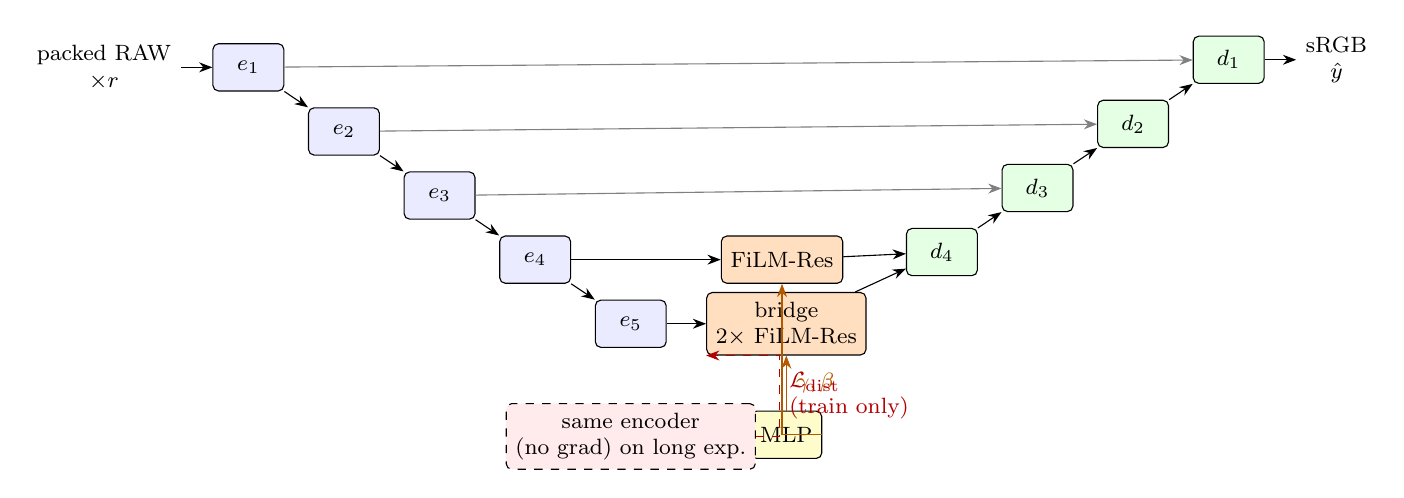
\begin{tikzpicture}[font=\footnotesize, >=Stealth,
  blk/.style={draw, rounded corners=2pt, minimum width=9mm, minimum height=6mm, fill=#1},
  blk/.default=gray!10]
\node[blk=blue!8] (e1) {$e_1$};
\node[blk=blue!8, below right=2mm and 3mm of e1] (e2) {$e_2$};
\node[blk=blue!8, below right=2mm and 3mm of e2] (e3) {$e_3$};
\node[blk=blue!8, below right=2mm and 3mm of e3] (e4) {$e_4$};
\node[blk=blue!8, below right=2mm and 3mm of e4] (e5) {$e_5$};
\node[blk=orange!25, right=5mm of e5, align=center] (br) {bridge\\$2\times$ FiLM-Res};
\node[blk=orange!25, right=19mm of e4] (sk) {FiLM-Res};
\node[blk=green!10, above right=2mm and 5mm of br] (d4) {$d_4$};
\node[blk=green!10, above right=2mm and 3mm of d4] (d3) {$d_3$};
\node[blk=green!10, above right=2mm and 3mm of d3] (d2) {$d_2$};
\node[blk=green!10, above right=2mm and 3mm of d2] (d1) {$d_1$};
\node[right=4mm of d1, align=center] (out) {sRGB\\$\hat y$};
\node[left=4mm of e1, align=center] (in) {packed RAW\\$\times r$};
\draw[->] (in) -- (e1);
\draw[->] (e1) -- (e2); \draw[->] (e2) -- (e3); \draw[->] (e3) -- (e4); \draw[->] (e4) -- (e5);
\draw[->] (e5) -- (br); \draw[->] (br) -- (d4);
\draw[->] (d4) -- (d3); \draw[->] (d3) -- (d2); \draw[->] (d2) -- (d1); \draw[->] (d1) -- (out);
\draw[->] (e4) -- (sk); \draw[->] (sk) -- (d4);
\draw[->, gray] (e3) -- (d3); \draw[->, gray] (e2) -- (d2); \draw[->, gray] (e1) -- (d1);
\node[blk=yellow!20, below=7mm of br, align=center] (mlp) {MLP};
\node[left=4mm of mlp, align=center] (c) {$(\log r,\ \log\hat\sigma)$};
\draw[->] (c) -- (mlp);
\draw[->, orange!70!black] (mlp) -- node[right] {$\gamma,\beta$} (br);
\draw[->, orange!70!black] (mlp.east) -| (sk.south);
\node[blk=red!8, below=7mm of e5, align=center, dashed] (te) {same encoder\\(no grad) on long exp.};
\draw[->, dashed, red!70!black] (te.east) -- ++(3mm,0) |- node[near start, right, align=left] {$\mathcal L_{\text{dist}}$\\(train only)} (br.south west);
\end{tikzpicture}}
\caption{Bridge U-Net. The SID encoder/decoder are unchanged. FiLM residual blocks refine the bottleneck $e_5$ and the skip $e_4$, conditioned on exposure ratio and estimated noise level. During training, features of the long exposure from the same encoder supervise the refined features (teacher-latent distillation).}
\label{fig:arch}
\end{figure}

\paragraph{Bottleneck refinement.} The bottleneck feature $e_5$ passes through $n_b=2$ residual blocks $e_5 \leftarrow e_5 + W_2\,\phi(\text{FiLM}(W_1 e_5))$. $W_2$ is zero-initialised, so the network starts exactly as the baseline. The 4th-level skip feature $e_4$ passes through one more such block before it reaches the decoder (``conditional skip refinement''). The plain U-Net instead copies the noisy $e_4$ straight into the decoder.

\paragraph{FiLM conditioning on the degradation.} The same network must handle $\times100$ to $\times300$ amplification and very different noise. We give it a two-number condition: the normalised log exposure ratio $\log r/\log 300$ and the log noise level $\hat\sigma$. $\hat\sigma$ is estimated from the input as the median absolute deviation of $G_1-G_2$, which removes scene content. An MLP maps the condition to a 64-d embedding, and each bridge block predicts its own $(\gamma,\beta)$ from it~\cite{perez2018film}.

\paragraph{Teacher-latent distillation.} During training only, the long-exposure RAW (packed and normalised the same way) goes through the \emph{same} encoder without gradient. Its features $t_4,t_5$ are what the encoder would produce from a clean input. We pull the refined student features towards them~\cite{romero2015fitnets,vapnik2009lupi}:
\begin{equation}
\mathcal{L}_{\text{dist}} = \tfrac12\sum_{l\in\{4,5\}} \frac{1}{|\Omega_l|}\sum_{p\in\Omega_l}\Big(1-\frac{\langle e_l(p), t_l(p)\rangle}{\|e_l(p)\|\,\|t_l(p)\|}\Big),
\end{equation}
the mean cosine distance between student and teacher feature vectors over all pixels $p$. The loss compares directions and not magnitudes, which differ between an amplified short exposure and a long exposure. (The first version used an L1 distance between normalised vectors, which is roughly $1/\sqrt{C}$ smaller per element and was negligible next to the image loss.) The full loss is
$\mathcal{L} = \|\hat y-y\|_1 + 0.1\,(1-\text{MS-SSIM}(\hat y,y))\,[\text{step}\ge s_0] + \lambda\mathcal{L}_{\text{dist}}$
with $\lambda=0.1$. MS-SSIM is switched on after $s_0$ steps, once the image is roughly right. At test time the long exposure is not needed. The model has \BRIDGEPARAMS{} parameters.

\subsection{Fine-tuning to new cameras}
\label{sec:ft}
To move a SID-trained model to the ELD cameras, we fine-tune all layers on every pair of scenes 1--6 of the three cameras (\ELDFTPAIRS{} pairs, all four ratios). We use AdamW (lr $5\times10^{-5}$), cosine decay, gradient clipping at 1, an EMA of the weights (decay 0.999) and the same loss as above. The variant \emph{decoder+bridge} freezes the encoder. Model selection uses the held-out scenes 7--10.

\subsection{Few-shot adaptation with meta-learning}
\label{sec:meta}
\paragraph{Question.} Full fine-tuning uses 6 scenes per camera. Can a model adapt to a new sensor from $K\in\{1,3,5\}$ scenes, and does meta-learning give a better starting point for that than ordinary supervised pre-training?

\paragraph{What went wrong in the first version.} The original project treated each SID \emph{scene} as a task, with 5 short exposures as support and up to 8 more from the same scene as query. Because all short exposures of a scene share one long-exposure target (Section~\ref{sec:data}), the query targets were already in the support set. The inner loop could memorise the answer, so the meta-objective did not measure adaptation. This explains why the curves in the original report stayed flat.

\paragraph{Task construction.} A task must differ from other tasks in something the model can learn from a few examples. It must also have a query that is \emph{not} in its support. On a new camera, what changes is mainly the colour response of the sensor (and its noise). We therefore simulate a new sensor per task:
\begin{itemize}
\item a sensor response $g=(g_R,g_G,g_B,g_G)$ with $\log g_c\sim\mathcal{U}(-0.35,0.35)$, multiplied into the packed RAW of both short and long exposures, while the sRGB target is left unchanged. The model must learn to undo an unknown colour transform;
\item one exposure ratio $r\in\{100,250,300\}$;
\item a support set of $K=5$ \emph{scenes} and a query set of $Q=8$ \emph{other} scenes, all drawn from the \SIDTRAINSCENES{} training scenes, with one random short exposure of ratio $r$ per scene and a random $256\times256$ packed crop.
\end{itemize}
The number of distinct tasks is effectively unlimited: $\binom{\SIDTRAINSCENES}{5}\binom{\SIDTRAINSCENES-5}{8}$ scene choices times a continuous gain space. We meta-train for \METAITERS{} outer steps with \METABATCH{} tasks each, i.e.\ \METATASKS{} sampled tasks covering every training scene many times. In the inner loop we take 3 SGD steps with $\alpha=10^{-3}$ on the support L1 loss. In the outer loop we use Adam (lr $10^{-5}$) on the query L1 loss through the adapted weights (second-order MAML, Eq.~\ref{eq:maml}), starting from the trained Bridge U-Net.

\paragraph{Meta-test.} The real test tasks are the three ELD cameras. For each camera and $K\in\{0,1,3,5\}$, the support set is all pairs of scenes $1..K$ (12 pairs per scene). We adapt with 200 Adam steps (lr $2\times10^{-5}$, batch 4, $512$ crops) and evaluate on the 24 test pairs of scenes 7--10, so support and query never share a scene. We compare three initialisations under the same adaptation: the SID U-Net, the Bridge U-Net and the meta-learned Bridge U-Net.

\subsection{Diffusion bridge models}
\label{sec:ddbm}
\paragraph{DDBM-Feature (the original variant).} The original project kept the Brownian bridge of Eq.~\ref{eq:bb}, but in feature space. For levels 3--5 of the encoder, the decoder receives $f_t=(1-t)f_{\text{short}}+t f_{\text{long}}+\sigma_{\max}\sqrt{t(1-t)}\,\epsilon$ with $\sigma_{\max}=0.1$ and $t\sim\mathcal U(0.01,0.99)$. A sinusoidal embedding of $t$ modulates every decoder block, and the network predicts the clean image directly with $\mathcal L_1+0.1(1-\text{MS-SSIM})$. At test time no long exposure exists. The output $y_{k-1}$ is mosaicked back to a pseudo-RAW, re-encoded as $f_{\text{long}}$ and decoded at $t_k=k/N$, for $N=3$ deterministic steps. No score is learned and the sampler is not a reverse diffusion, so this is a time-conditioned U-Net with feature mixing as augmentation rather than a DDBM.

\paragraph{DDBM (pixel space, new).} We also implement the actual model of~\cite{zhou2024ddbm} with a VE/Brownian-bridge schedule. The endpoints are the target $x_0=2y-1$ and a \emph{naive rendering} of the input, $x_T$: the amplified packed RAW with averaged greens, camera white balance, gamma $1/2.2$ and bilinear $2\times$ up-sampling, in $[-1,1]$. With $T=1$ and $\sigma^2=0.5$, Eq.~\ref{eq:bb} gives $x_t$. A time-conditioned U-Net $D_\theta(x_t,t,x_T,\text{RAW})$ (pixel-unshuffled inputs, channels $\{64,\dots,512\}$, \DDBMPARAMS{} parameters) predicts $x_0$. Its loss $\|D_\theta-x_0\|^2$ is denoising bridge score matching in the $x_0$-parameterisation, since the bridge score is $\big((1-t)D_\theta+tx_T-x_t\big)/(\sigma^2t(1-t))$. To sample, we walk $t$ from 1 to 0 in $N$ steps. Each step draws from the exact posterior of a Brownian bridge pinned at $\hat x_0=D_\theta$ and the current state:
\begin{equation}
x_s \mid x_t,\hat x_0 \sim \mathcal N\!\Big((1-\tfrac st)\hat x_0 + \tfrac st x_t,\ \sigma^2\tfrac{s(t-s)}{t}I\Big),
\end{equation}
which is the ancestral sampler ($\eta=1$). The deterministic DBIM sampler~\cite{zheng2025dbim} ($\eta=0$) reuses the predicted noise instead. Table~\ref{tab:ddbmcmp} contrasts the two bridge variants.

\paragraph{DDBM with the released recipe.} The model above is a simplified DDBM: a small bridge variance, an unweighted $x_0$ loss and a first-order sampler. To check that these simplifications do not explain our findings, we also train the recipe of the released DDBM code~\cite{zhou2024ddbm}, which follows EDM~\cite{karras2022edm}. The bridge is a VE bridge indexed by the noise level $\sigma\in[\sigma_{\min},\sigma_{\max}]$, with marginal
\begin{equation}
x_\sigma = a\,x_T + (1-a)\,x_0 + \sigma\sqrt{1-a}\;\epsilon,\qquad a=\sigma^2/\sigma_{\max}^2 .
\end{equation}
The network is wrapped in the EDM preconditioning
\begin{equation}
D_\theta = c_{\text{skip}}(\sigma)\,x_\sigma + c_{\text{out}}(\sigma)\,F_\theta\big(c_{\text{in}}(\sigma)x_\sigma,\ \tfrac14\log\sigma,\ x_T,\text{RAW}\big),
\end{equation}
where $c_{\text{in}},c_{\text{skip}},c_{\text{out}}$ give unit-variance inputs and targets for $\sigma_{\text{data}}=0.5$. The loss is weighted by $\lambda(\sigma)=1/c_{\text{out}}(\sigma)^2$ and $\sigma\sim\mathcal U(\sigma_{\min},\sigma_{\max})$. Sampling uses the hybrid sampler of DDBM on a Karras schedule ($\rho=7$): each step is a stochastic Euler--Maruyama step of the bridge SDE over a fraction $0.33$ of the interval, followed by a Heun step of the probability-flow ODE, whose drift contains the Doob $h$-transform term $\nabla\log p(x_T\mid x_\sigma)=(x_T-x_\sigma)/(\sigma_{\max}^2-\sigma^2)$. $N$ steps cost $3N-1$ network evaluations. We use the same network $F_\theta$ as above and train two versions: the released default $\sigma_{\max}=80$ (60k steps) and $\sigma_{\max}=1$ (30k steps), which matches the noise scale to the $[-1,1]$ data range. Everything else is identical.

\begin{table}[t]
\centering
\caption{The three diffusion-bridge variants compared in this report.}
\label{tab:ddbmcmp}
\small
\resizebox{\linewidth}{!}{%
\begin{tabular}{@{}llll@{}}
\toprule
 & DDBM-Feature & DDBM (simplified) & DDBM (released recipe) \\
\midrule
space & encoder features & pixels (sRGB) & pixels (sRGB) \\
endpoints & short / long features & $x_T$ = naive render, $x_0$ = GT & same \\
bridge & BB, $\sigma_{\max}=0.1$ & BB, $\sigma^2=0.5$ & VE, $\sigma_{\max}\in\{80,1\}$ \\
network output & image & $x_0$ & EDM-preconditioned $x_0$ \\
loss & $\mathcal L_1$ + MS-SSIM & $\|D-x_0\|^2$ & $\lambda(\sigma)\|D-x_0\|^2$ \\
score learned & no & yes & yes \\
sampler & re-encode, $N=3$ & bridge posterior / DBIM & Euler--Maruyama + Heun \\
NFE for $N$ steps & $N+1$ & $N$ & $3N-1$ \\
\bottomrule
\end{tabular}}
\end{table}

\section{Experiments}
\label{sec:exp}

\subsection{Setup}
\label{sec:setup}
All models were trained and evaluated on one NVIDIA A100 (80\,GB) on Google Colab, with bf16 mixed precision. The supervised models (SID U-Net, Bridge U-Net and its ablations, DDBM-Feature) use AdamW with learning rate $2\times10^{-4}$, a 500-step warm-up, cosine decay to 2\%, batch 8, $512\times512$ packed crops and 40k iterations. MS-SSIM enters the loss after 20k iterations. Every 2k iterations we evaluate an EMA of the weights (decay 0.999) on 60 validation pairs (centre $512\times512$ packed crop), and we test the best validation checkpoint. The pixel-space DDBMs use learning rate $10^{-4}$ (1k-step warm-up, then constant), batch 16, $256\times256$ crops and are validated on 20 pairs with $N=10$ steps. Besides the fidelity metrics PSNR, SSIM and MS-SSIM we report LPIPS~\cite{zhang2018lpips} (AlexNet, lower is better) on the full-resolution images, a learned perceptual distance that, unlike PSNR, does not reward a blurry average. Unless stated otherwise, \textbf{test numbers are on all \SIDTESTPAIRS{} SID test pairs at full resolution} ($4256\times2848$), not on crops. Each configuration was trained once (one seed). To estimate run-to-run variation we retrained the SID U-Net with a second seed (Section~\ref{sec:sidres}).

One practical note: the first Bridge U-Net run diverged after 2.5k iterations (the loss jumped from 0.05 to 0.4 and never recovered). We restarted it and, for all runs, skip a batch whose loss exceeds five times the running average after the first 1k iterations (at most 10 in a row), which happened only a handful of times.

\subsection{SID: baseline, Bridge U-Net and ablations}
\label{sec:sidres}

\begin{table}[t]
\centering
\caption{SID Sony test set (\SIDTESTPAIRS{} full-resolution pairs). NFE: network evaluations per image; time: seconds per full-resolution image on an A100 (network only). LPIPS was added after the first set of checkpoints was lost, so it is measured on retrained copies ($^\dagger$: same configuration and seed; the copies score 28.61, 27.97 and 27.88\,dB PSNR, within 0.06\,dB of the original runs). The best value per column is in bold.}
\label{tab:sid}
\small
\resizebox{\linewidth}{!}{%
\begin{tabular}{@{}lrrccccr@{}}
\toprule
Model & Params & NFE & PSNR$\uparrow$ & SSIM$\uparrow$ & MS-SSIM$\uparrow$ & LPIPS$\downarrow$ & Time (s) \\
\midrule
SID U-Net, reported in~\cite{chen2018sid} & 7.8M & 1 & 28.88 & 0.787 & -- & -- & -- \\
SID U-Net (ours) & \PSID & 1 & 28.62 & 0.796 & \textbf{0.876} & \SIDRELPIPS$^\dagger$ & \TSID \\
SID U-Net (ours, second seed) & \PSID & 1 & \SIDRERUNPSNR & \SIDRERUNSSIM & \SIDRERUNMS & -- & \\
\midrule
Bridge U-Net (FiLM + distillation) & \PBRIDGE & 1 & 28.36 & 0.789 & 0.868 & -- & \TBRIDGE \\
\quad w/o distillation & \PBRIDGE & 1 & \textbf{28.94} & \textbf{0.798} & \textbf{0.876} & -- & \TBRIDGE \\
\quad w/o FiLM & \PNOFILM & 1 & 28.11 & 0.787 & 0.868 & -- & \TNOFILM \\
\midrule
DDBM-Feature, iterative ($N=3$) & \PFEAT & 4 & 18.02 & 0.449 & 0.742 & -- & \TFEATTHREE \\
DDBM-Feature, single pass & \PFEAT & 1 & 25.51 & 0.733 & 0.841 & -- & \TFEATZERO \\
DDBM, simplified, $N=5$ & \PDDBM & 5 & 28.03 & 0.782 & 0.862 & \textbf{\DDBMREFIVELPIPS}$^\dagger$ & \TDDBMFIVE \\
DDBM, simplified, $N=10$ & \PDDBM & 10 & 27.90 & 0.779 & 0.856 & \textbf{\DDBMRETENLPIPS}$^\dagger$ & \TDDBMTEN \\
DDBM, simplified, $N=10$, $\eta=0$ & \PDDBM & 10 & 27.88 & 0.776 & 0.854 & -- & \TDDBMTEN \\
DDBM, simplified, $N=20$ & \PDDBM & 20 & 27.77 & 0.776 & 0.851 & -- & \\
DDBM, released recipe, $\sigma_{\max}=1$, $N=5$ & \PDDBM & 14 & \SONEFIVEPSNR & \SONEFIVESSIM & \SONEFIVEMS & \SONEFIVELPIPS & \TOFFFIVE \\
DDBM, released recipe, $\sigma_{\max}=1$, $N=10$ & \PDDBM & 29 & \SONETENPSNR & \SONETENSSIM & \SONETENMS & \SONETENLPIPS & \TOFFTEN \\
DDBM, released recipe, $\sigma_{\max}=1$, $N=20$ & \PDDBM & 59 & \SONETWENTYPSNR & \SONETWENTYSSIM & \SONETWENTYMS & \SONETWENTYLPIPS & \\
\bottomrule
\end{tabular}}
\end{table}

Table~\ref{tab:sid} gives the main results. Our SID U-Net reaches 28.62\,dB, 0.26\,dB below the original paper~\cite{chen2018sid} and with a higher SSIM. The paper trains for 4000 epochs and we train for 40k iterations of batch 8, so the reproduction is faithful. A second training run with a different seed gives \SIDRERUNPSNR\,dB (SSIM \SIDRERUNSSIM), a difference of only \SIDSEEDGAP\,dB on the test set (33.07 vs.\ 32.89\,dB on validation). Two runs are a weak estimate of the variance, but they suggest that the test-set gaps of 0.25\,dB and more discussed below are not run-to-run noise.

\paragraph{The bridge module.} With both FiLM and distillation, the Bridge U-Net (28.36\,dB) is slightly \emph{worse} than the baseline. The ablations show why. Removing FiLM costs a further 0.25\,dB, so conditioning on exposure ratio and noise level helps. Removing distillation \emph{gains} 0.58\,dB, and the Bridge U-Net without distillation is the best model of this report: 28.94\,dB, +0.32\,dB over the baseline. The same order holds on the validation set (33.17 vs.\ 33.07\,dB for SID and 32.35\,dB with distillation). The distillation loss itself stays small, around $3\times10^{-4}$ in cosine distance: the encoder already maps the amplified short exposure and the long exposure to features of nearly the same direction. The loss therefore does little to clean the features. What it does do is pull the output of the bridge blocks back towards the plain encoder features, which removes most of the freedom the bridge was added for. In our setting, teacher-latent distillation is a regulariser that hurts.

\subsection{Diffusion bridges}
\label{sec:ddbmres}

\begin{figure}[t]
\centering
\begin{tikzpicture}
\begin{axis}[width=0.95\linewidth, height=5.2cm, xlabel={training iteration}, ylabel={val PSNR (dB)},
  xmin=0, xmax=60000, ymin=10, ymax=34, grid=major, grid style={gray!25},
  legend pos=south east, legend style={font=\footnotesize}, scaled x ticks=false,
  xtick={0,10000,20000,30000,40000,50000,60000}, xticklabels={0,10k,20k,30k,40k,50k,60k}]
\addplot[black, thick, mark=none] table[x=step,y=psnr] {data/val_sid.dat};
\addplot[blue, thick, mark=none] table[x=step,y=psnr] {data/val_ddbm.dat};
\addplot[red, thick, mark=none] table[x=step,y=psnr] {data/val_ddbm_official.dat};
\addplot[orange, thick, mark=none] table[x=step,y=psnr] {data/val_ddbm_official_s1.dat};
\legend{SID U-Net, DDBM simplified, DDBM released $\sigma_{\max}=80$, DDBM released $\sigma_{\max}=1$}
\end{axis}
\end{tikzpicture}
\caption{Validation PSNR during training (20--60 SID validation pairs, centre crops, $N=10$ sampling steps for the DDBMs). With the released noise scale $\sigma_{\max}=80$ the DDBM learns very slowly. Matching the noise scale to the data ($\sigma_{\max}=1$) speeds up training a lot, but after 60k iterations the recipe still trails the simplified DDBM by about 4\,dB on validation (27.0 vs.\ 31.2--31.4\,dB).}
\label{fig:valcurves}
\end{figure}

\paragraph{DDBM-Feature does not work as a diffusion model.} The feature-space variant of the original project reaches 25.51\,dB when it is run as a single pass at $t=0$, i.e.\ as a time-conditioned U-Net. Its intended iterative inference, which re-encodes its own output as the ``long exposure'' feature, collapses to 18.02\,dB. During training the decoder always sees features of the \emph{true} long exposure, while at test time it sees features of its own previous estimate, so errors compound from step to step. The longer we train, the more the decoder relies on these features: the validation PSNR of the iterative sampler peaks at 19.7\,dB after 6k iterations and falls to 12.3\,dB at 40k. A bridge whose endpoint is unavailable at test time cannot be sampled this way. This is why we implemented the pixel-space model, whose endpoint $x_T$ comes from the input itself.

\paragraph{A real DDBM is competitive but does not beat regression on PSNR.} The simplified pixel-space DDBM reaches 28.03\,dB with $N=5$ steps, 0.6\,dB below the SID U-Net, with twice the parameters and five times the compute. More sampling steps make it \emph{worse}: 27.90\,dB at $N=10$ and 27.77\,dB at $N=20$. This is expected. PSNR and SSIM reward the posterior mean, which is exactly what an $L_1$/$L_2$ regression network estimates. A diffusion model is trained to draw \emph{samples} from the posterior, and for an exact sampler the expected squared error of a sample is twice that of the posterior mean. Fewer steps behave more like a single denoising step and stay closer to the mean, so they score higher. The deterministic DBIM sampler ($\eta=0$) gives the same PSNR as the ancestral one. The possible benefit of diffusion, sharper texture instead of a blurry average, is not what these metrics measure.

\paragraph{On a perceptual metric the DDBM is better.} LPIPS reverses the order. The simplified DDBM scores \DDBMREFIVELPIPS{} against \SIDRELPIPS{} for the SID U-Net, 14\% lower, while being 0.6\,dB worse in PSNR. This is the perception--distortion trade-off~\cite{blau2018perception}: no estimator can be best on both, and the regression network sits at the low-distortion end. Unlike PSNR, LPIPS does not get worse with more steps ($N=5$ and $N=10$ give the same value), so the extra steps move the output away from the mean without making it look less like the target. The released recipe shows the same effect more strongly. From $N=10$ to $N=20$ its LPIPS improves from \SONETENLPIPS{} to \SONETWENTYLPIPS{}, almost reaching the simplified model, although its PSNR (\SONETWENTYPSNR\,dB) stays 2.4\,dB lower. The gain is modest in the crops of Fig.~\ref{fig:crops}: the simplified DDBM looks much like the U-Net, slightly less smooth in flat regions, and in the $\times250$ scene its colours drift towards yellow. Because LPIPS was measured on retrained copies, this comparison rests on one run per model.

\paragraph{The released recipe: the noise scale explains the slow start, not the gap.} Trained with its default $\sigma_{\max}=80$ for 60k iterations, the released DDBM recipe reached only 24.09\,dB on validation (SSIM 0.405), against 31.43\,dB for the simplified DDBM with the same network (Fig.~\ref{fig:valcurves}). Its validation PSNR stayed at about 12\,dB for the first 20k iterations. We traced this to the noise scale. Our images lie in $[-1,1]$, while the bridge noise at $\sigma=\sigma_{\max}/\sqrt2$ has a standard deviation of about 40, so in the middle of the bridge $x_\sigma$ is almost pure noise. And because $\sigma\sim\mathcal U(\sigma_{\min},\sigma_{\max})$, 99\% of the training samples have $\sigma>0.8$, so the low-noise range that decides the final detail is rarely trained. These settings come from image-to-image translation, where the two endpoints differ a lot. With $\sigma_{\max}=1$ and everything else unchanged, training is much faster: 21.4\,dB after 4k iterations and 25.85\,dB after 30k, against 12.5 and 17.0\,dB for $\sigma_{\max}=80$ at the same points. We then retrained it for the full 60k iterations, where it reaches \SONEVAL\,dB on validation, about 3\,dB above $\sigma_{\max}=80$ at the same point. The test score is still far below the simplified DDBM: \SONEFIVEPSNR, \SONETENPSNR{} and \SONETWENTYPSNR\,dB with $N=5$, 10 and 20, with low SSIM (\SONEFIVESSIM--\SONETWENTYSSIM). Two observations point to the sampler rather than the network. First, more steps help here, the opposite of the simplified model, and the gain has not levelled off at $N=20$. Second, the outputs keep visible residual noise and invented texture, and they are darker with a colour shift (Fig.~\ref{fig:crops}). With the stochastic churn step and the Karras schedule, a handful of steps does not remove the injected noise, while the simplified model's bridge posterior lands exactly on $\hat x_0$ in its last step. For restoration, where $x_T$ is already close to $x_0$, a small-noise bridge with a sampler that ends on the denoised estimate (I$^2$SB~\cite{liu2023i2sb}, our simplified model) is the better fit. The test evaluation of the $\sigma_{\max}=80$ model was lost when the cloud machine was reclaimed, so we report its validation score only.

\begin{figure*}[t]
\centering
\setlength{\tabcolsep}{1pt}
\begin{tabular}{ccccc}
\footnotesize Input (amplified) & \footnotesize SID U-Net & \footnotesize DDBM, simplified & \footnotesize DDBM, released, $\sigma_{\max}=1$ & \footnotesize Ground truth \\

\includegraphics[width=0.186\linewidth]{fig/0_input_amp.jpg} &
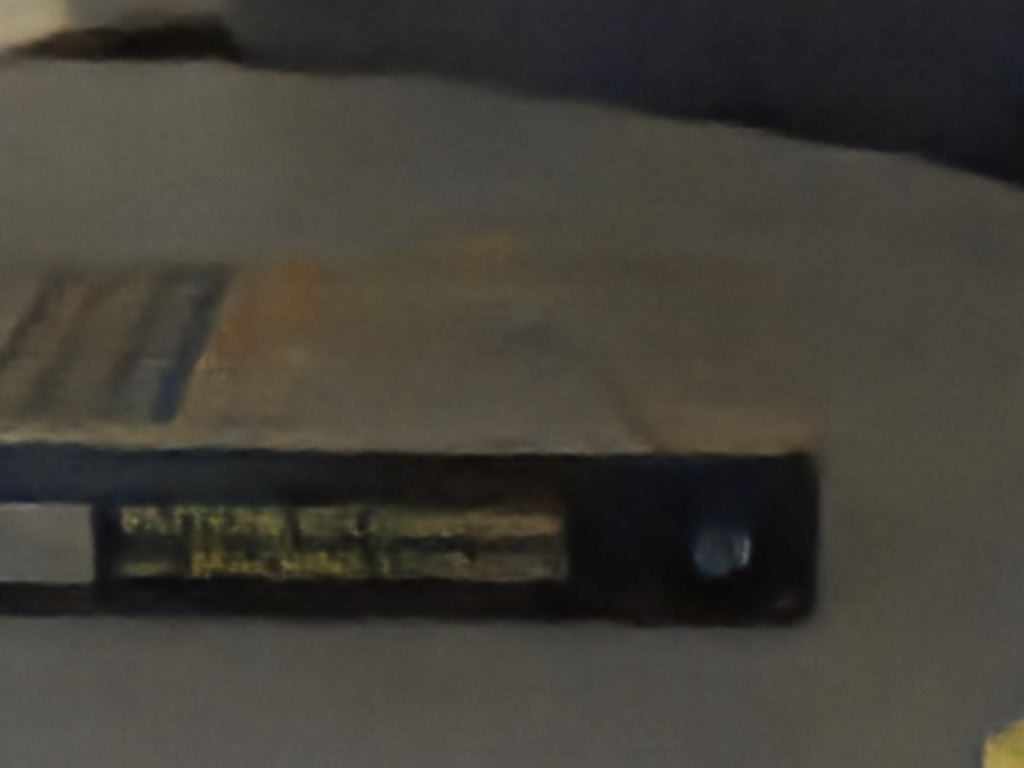
\includegraphics[width=0.186\linewidth]{fig/0_sid.jpg} &
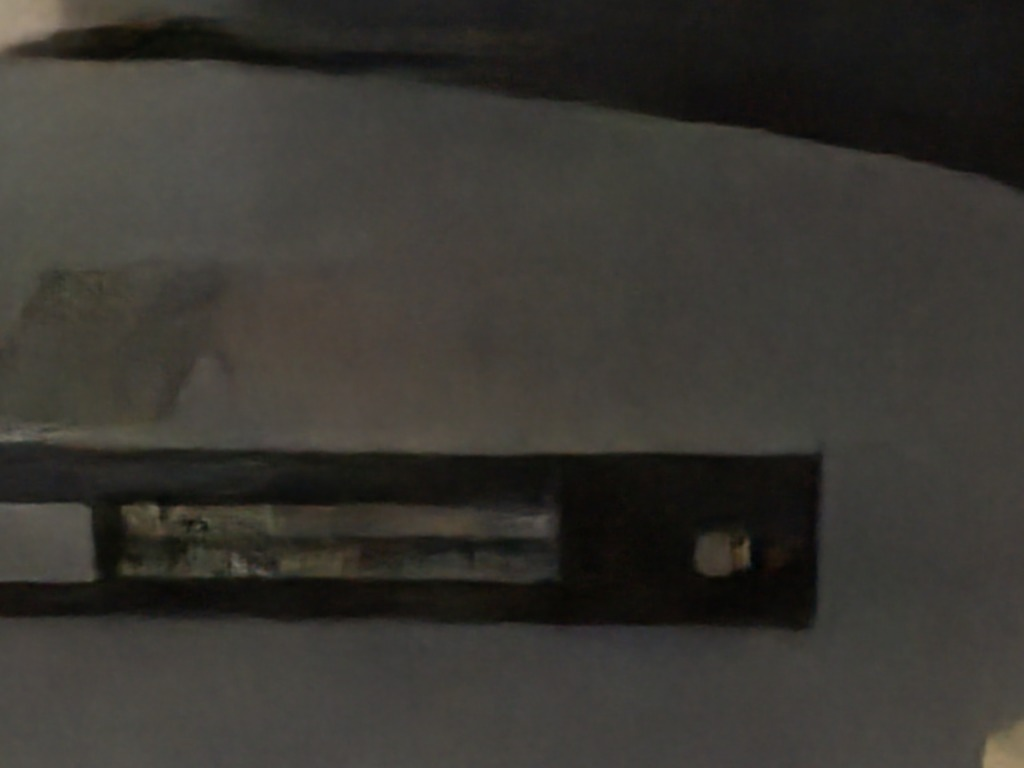
\includegraphics[width=0.186\linewidth]{fig/0_ddbm.jpg} &
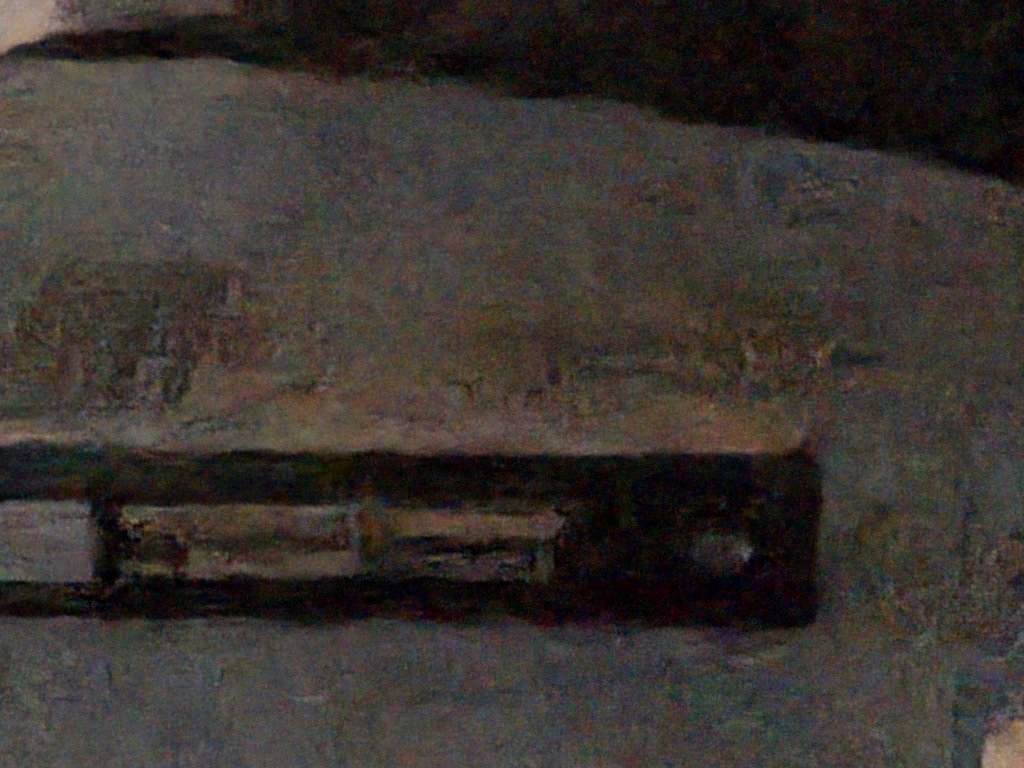
\includegraphics[width=0.186\linewidth]{fig/0_ddbm_official_s1.jpg} &
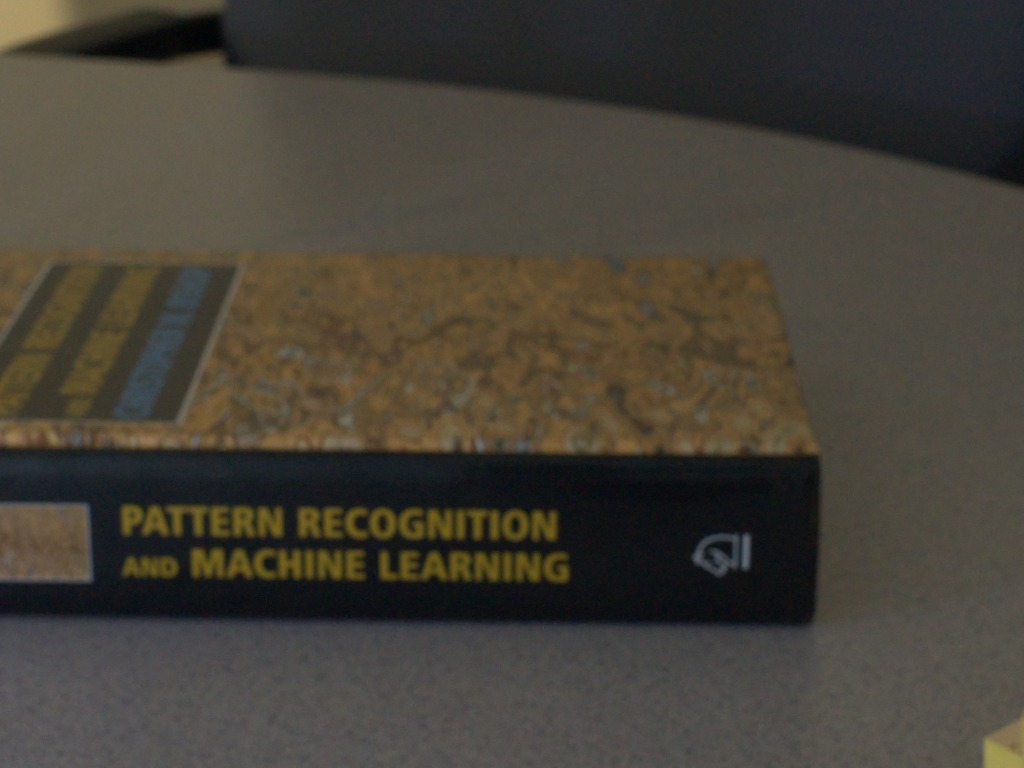
\includegraphics[width=0.186\linewidth]{fig/0_gt.jpg} \\
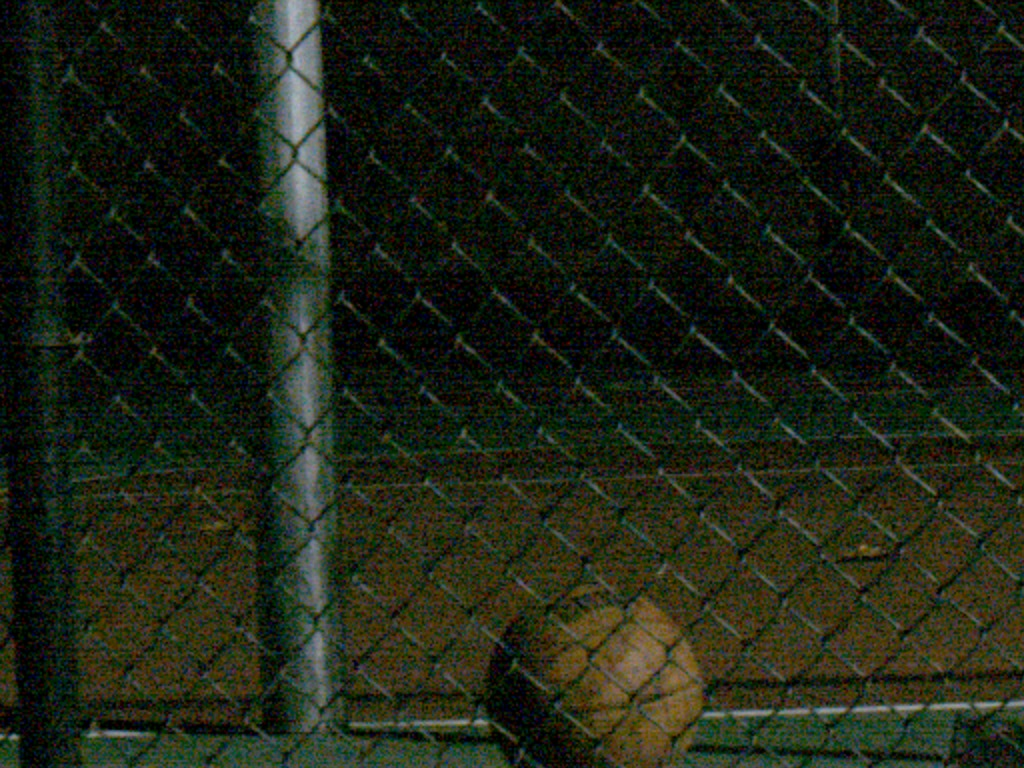
\includegraphics[width=0.186\linewidth]{fig/2_input_amp.jpg} &
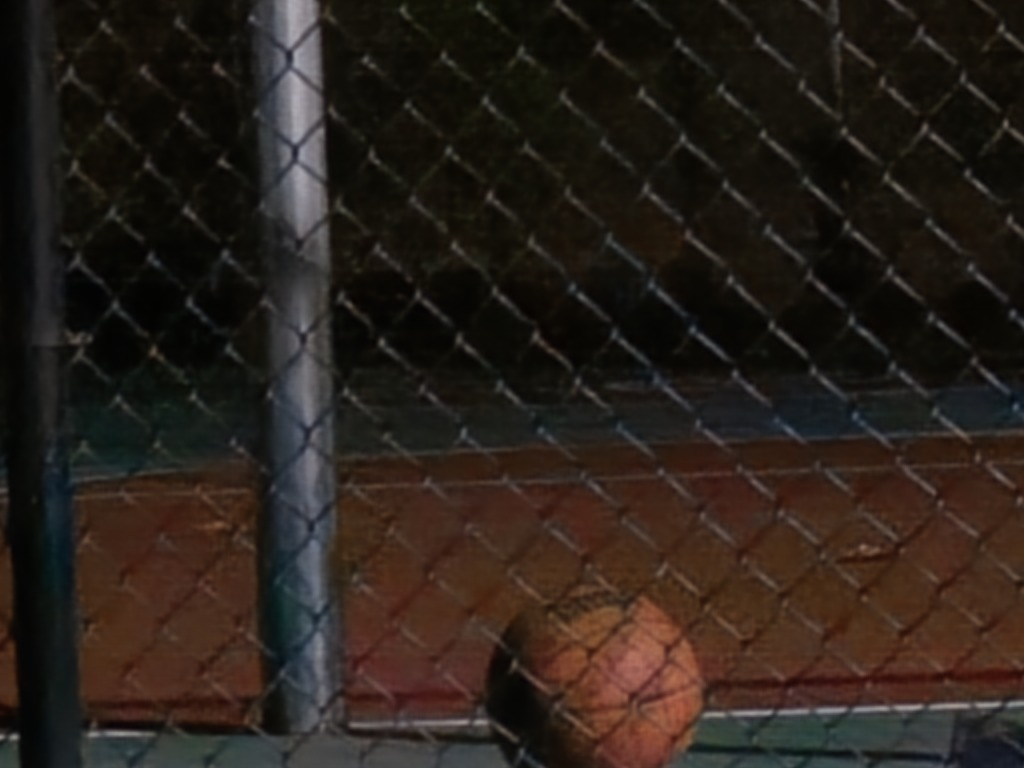
\includegraphics[width=0.186\linewidth]{fig/2_sid.jpg} &
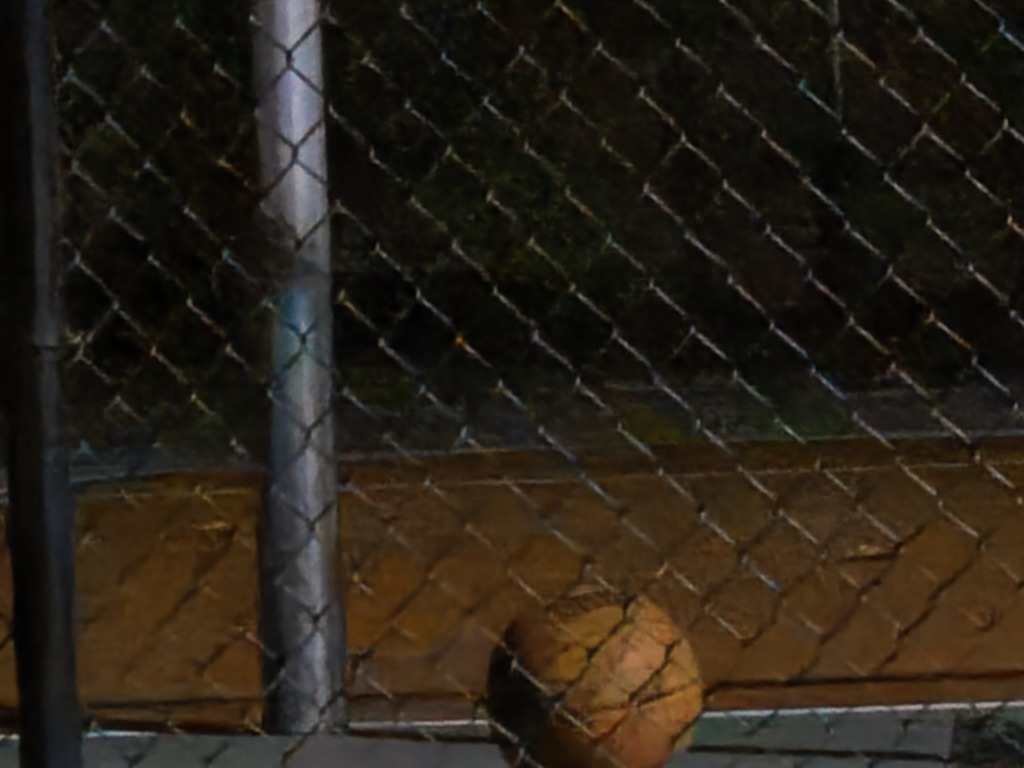
\includegraphics[width=0.186\linewidth]{fig/2_ddbm.jpg} &
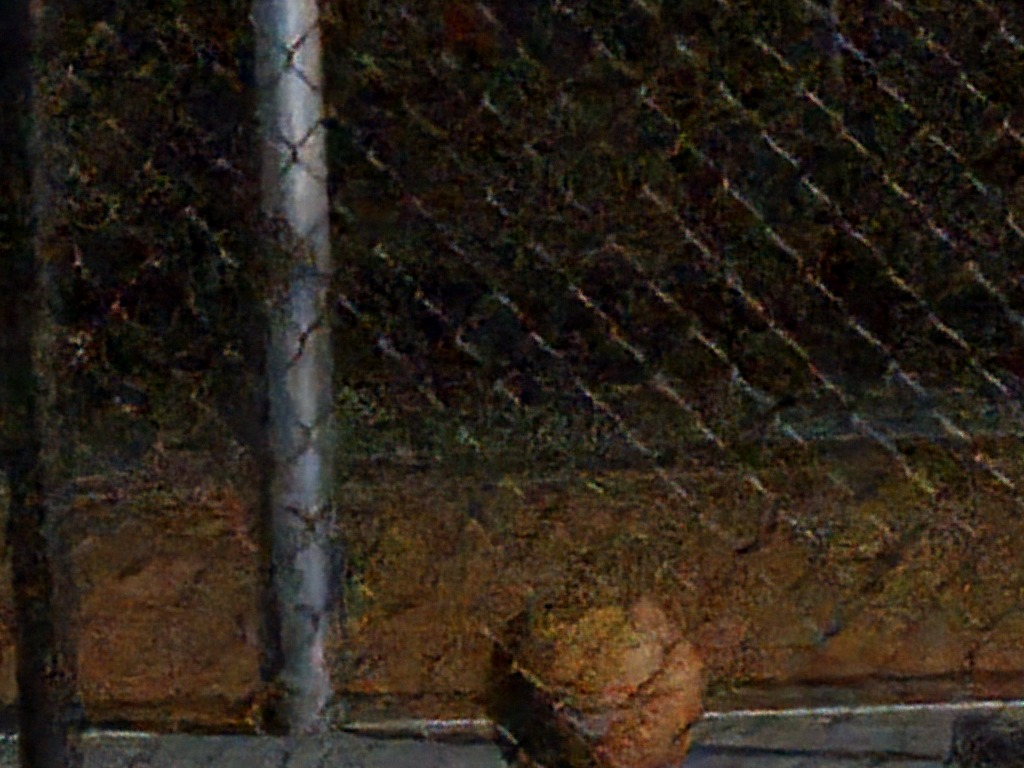
\includegraphics[width=0.186\linewidth]{fig/2_ddbm_official_s1.jpg} &
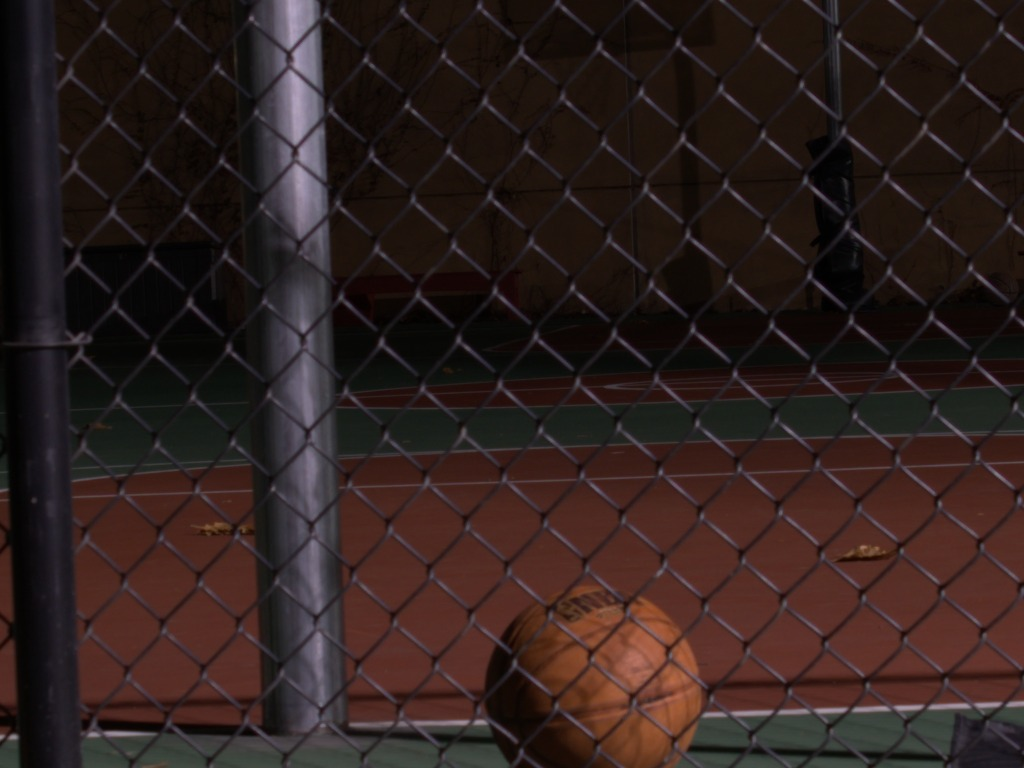
\includegraphics[width=0.186\linewidth]{fig/2_gt.jpg} \\
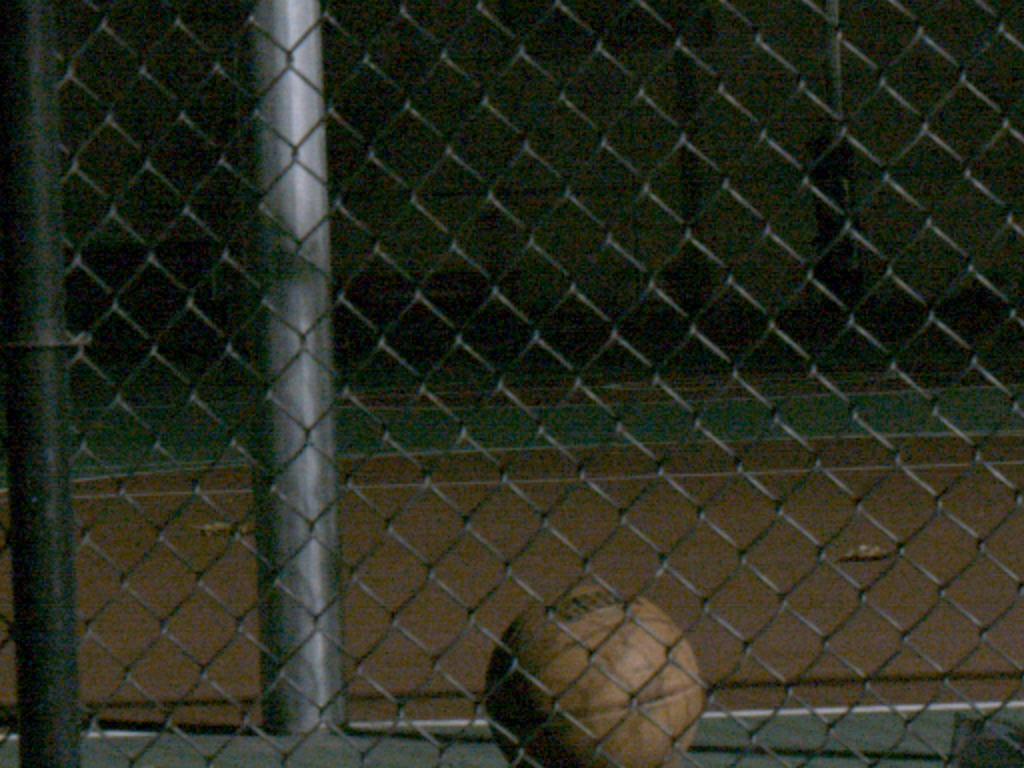
\includegraphics[width=0.186\linewidth]{fig/4_input_amp.jpg} &
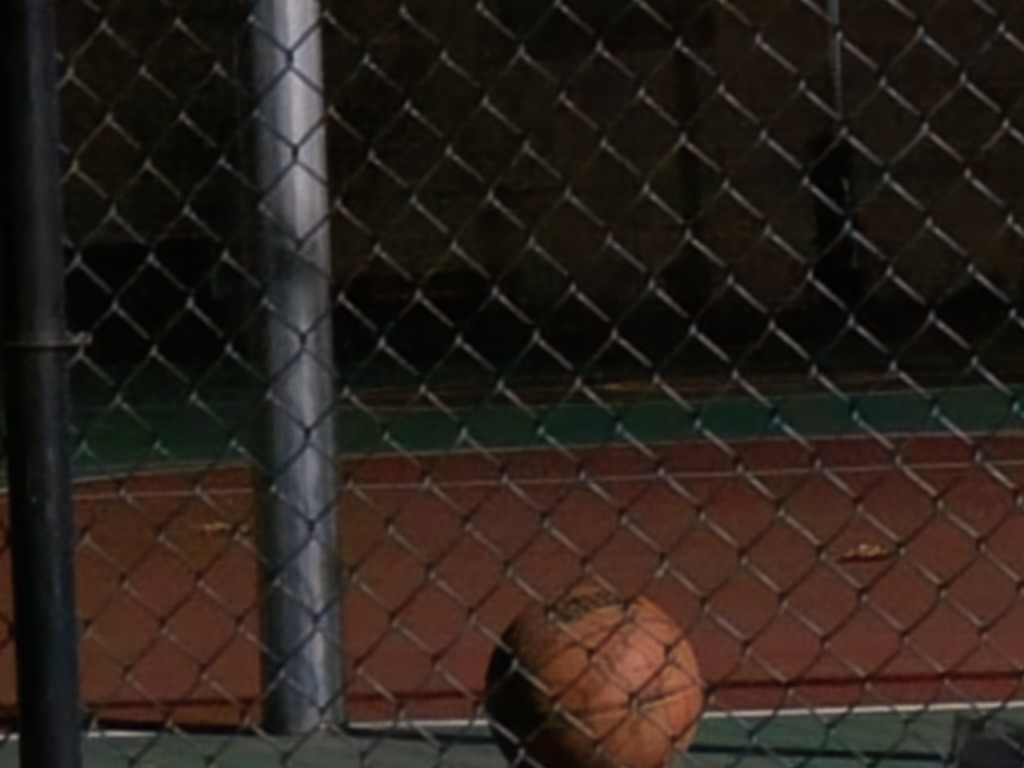
\includegraphics[width=0.186\linewidth]{fig/4_sid.jpg} &
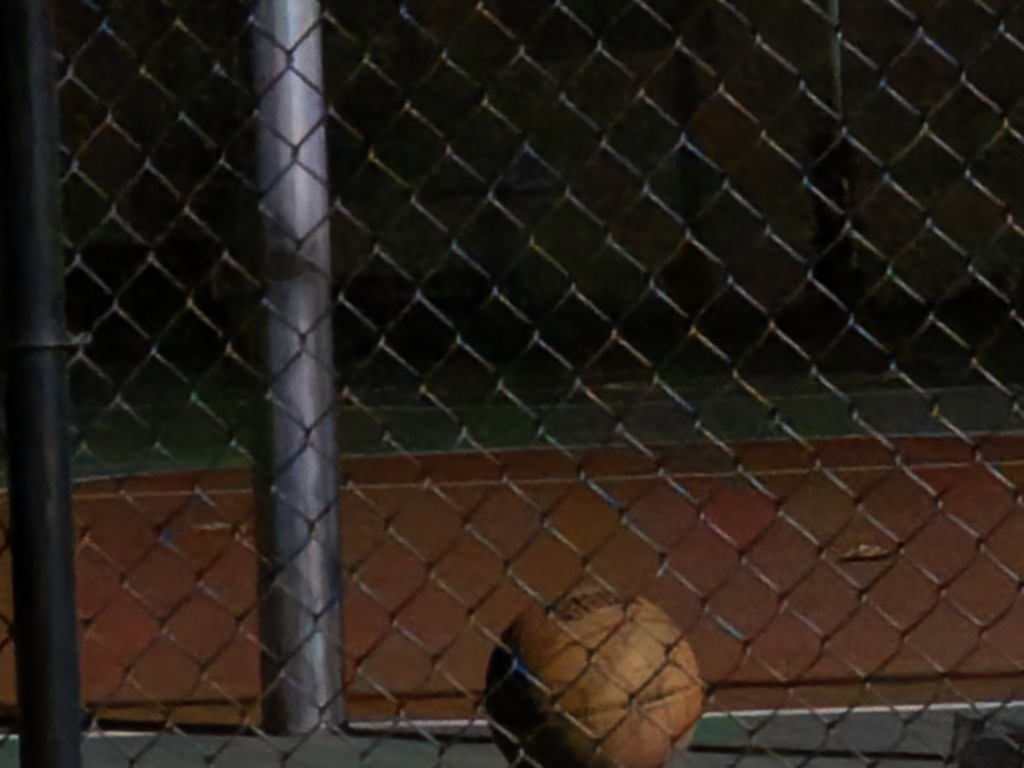
\includegraphics[width=0.186\linewidth]{fig/4_ddbm.jpg} &
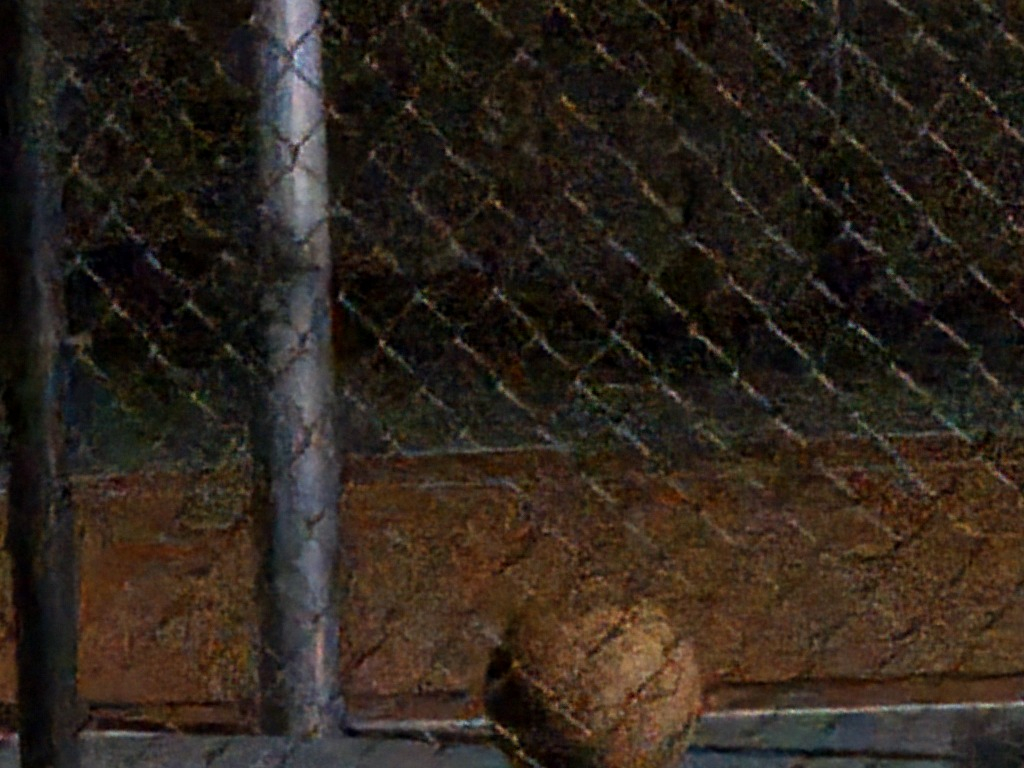
\includegraphics[width=0.186\linewidth]{fig/4_ddbm_official_s1.jpg} &
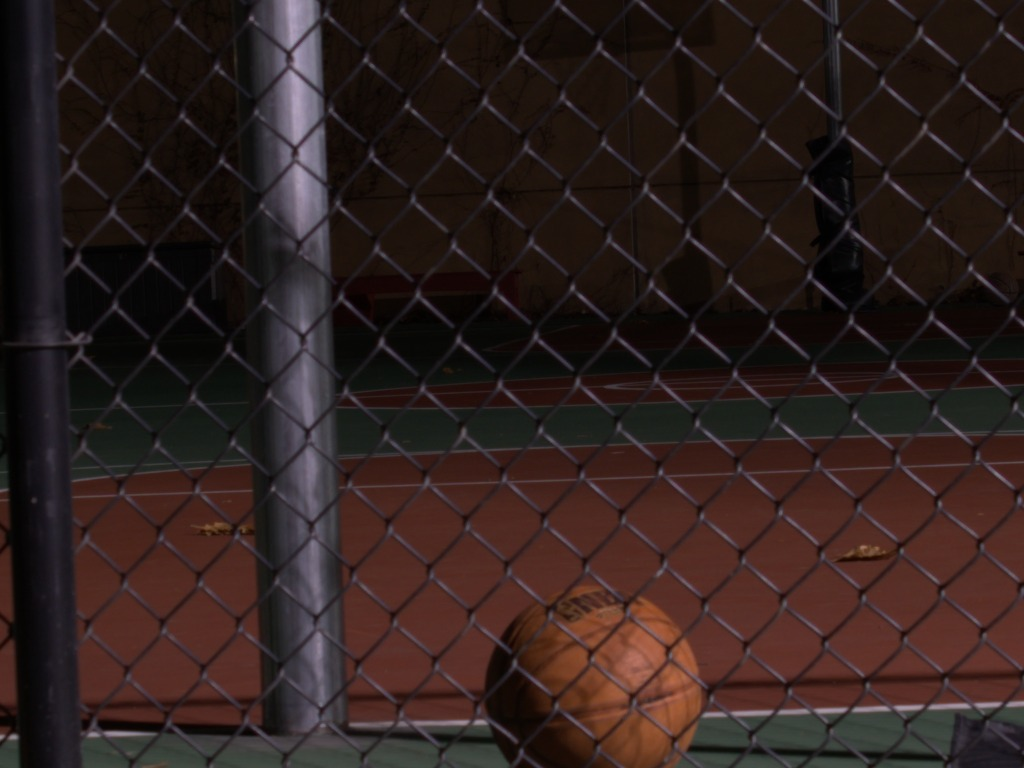
\includegraphics[width=0.186\linewidth]{fig/4_gt.jpg} \\
\end{tabular}
\caption{SID test crops ($1024\times768$ from the image centre) at exposure ratios $\times300$, $\times250$ and $\times100$ (top to bottom), from the models retrained after the first set of checkpoints was lost; both DDBMs use $N=10$ steps. The input is the amplified short exposure with a naive demosaic and white balance. The SID U-Net is smooth but faithful. The simplified DDBM is close to it, with a yellow colour drift in the middle row. The DDBM trained with the released recipe keeps residual noise, invents texture (the book cover) and is darker than the target.}
\label{fig:crops}
\end{figure*}

\subsection{Adapting to new cameras}
\label{sec:eldres}

\begin{table}[t]
\centering
\caption{ELD test scenes 7--10 ($\times100$ and $\times200$, 24 pairs per camera, $1024\times1024$ packed crops). PSNR / SSIM, starting from the SID-trained Bridge U-Net, which scores 24.37\,dB on average without adaptation. Fine-tuning uses all pairs of scenes 1--6 of the three cameras.}
\label{tab:eld}
\small
\begin{tabular}{@{}lcccc@{}}
\toprule
 & Canon 70D & Canon 700D & Nikon D850 & Mean \\
\midrule
Decoder + bridge & \textbf{26.16} / 0.740 & 25.99 / 0.709 & 29.35 / 0.811 & 27.17 / 0.753 \\
All layers & 26.14 / \textbf{0.745} & \textbf{26.01} / \textbf{0.713} & \textbf{29.81} / \textbf{0.827} & \textbf{27.32} / \textbf{0.762} \\
\bottomrule
\end{tabular}
\end{table}

\paragraph{Fine-tuning.} Without adaptation, the SID-trained model loses more than 4\,dB on the ELD cameras (24.37\,dB on average, against 28.4\,dB on SID). The other sensors have different colour responses and noise, and their frames span ratios down to $\times1$. Fine-tuning on the \ELDFTPAIRS{} pairs of scenes 1--6 recovers about 3\,dB (Table~\ref{tab:eld}): 27.32\,dB on average for all layers and 27.17\,dB with a frozen encoder. Freezing the encoder is almost as good on the two Canons and 0.46\,dB worse on the Nikon D850. Most of the camera-specific change can thus be absorbed by the decoder and the bridge, but low-level features still matter for a sensor that differs more from the Sony.

\begin{table}[t]
\centering
\caption{Few-shot adaptation on ELD: PSNR on scenes 7--10, averaged over the three cameras. $K$ adaptation scenes per camera, 12 pairs per scene. \emph{Adam}: 200 Adam steps (lr $2\times10^{-5}$); \emph{inner}: 30 SGD steps with the meta-training inner learning rate $10^{-3}$.}
\label{tab:fewshot}
\small
\begin{tabular}{@{}llcccc@{}}
\toprule
Initialisation & Adaptation & $K=0$ & $K=1$ & $K=3$ & $K=5$ \\
\midrule
SID U-Net & Adam & 24.17 & \textbf{26.74} & \textbf{27.36} & \textbf{27.54} \\
Bridge U-Net & Adam & 24.37 & 26.31 & 26.66 & 27.05 \\
Meta-learned Bridge & Adam & \textbf{24.77} & 26.48 & 26.86 & 27.15 \\
\midrule
Bridge U-Net & inner & -- & 24.40 & 24.53 & 24.25 \\
Meta-learned Bridge & inner & -- & \textbf{25.29} & \textbf{25.26} & \textbf{25.46} \\
\bottomrule
\end{tabular}
\end{table}

\paragraph{Few-shot adaptation and meta-learning.} Table~\ref{tab:fewshot} answers the second question. One scene of a new camera (12 pairs) already gives +1.7 to +2.6\,dB. Five scenes per camera (27.05--27.54\,dB) are as good as fine-tuning on six scenes of all three cameras (27.32\,dB). The meta-learned initialisation helps in two cases. It is the best model \emph{before} any adaptation ($K=0$: +0.40\,dB over the Bridge U-Net it started from and +0.60\,dB over SID), because meta-training on random sensor gains makes it robust to colour shifts. It is also clearly better when adaptation is as short as in meta-training (\emph{inner}: +0.9 to +1.2\,dB at every $K$). During meta-training the query loss after adaptation (L1 0.0459) was below the support loss before adaptation (0.0510), so the inner loop learned to adapt. With a long adaptation of 200 Adam steps, however, the advantage over the Bridge U-Net shrinks to 0.1--0.2\,dB, and the plain SID U-Net adapts best for every $K\ge1$. A good initialisation matters most when the adaptation budget is small. With more steps the initialisation matters less, and the smaller network (\PSID{} instead of \PBRIDGE{} parameters) adapts best from little data. The inner-loop adaptation does not improve with $K$, because 30 steps are too few to use more data.

\section{Conclusion}
\label{sec:conclusion}

We rebuilt the project from its first report, retrained every model and evaluated on the full-resolution SID test set and on held-out ELD scenes. The answers to the three questions are more nuanced than the first version suggested.

\begin{enumerate}
\item \textbf{Bottleneck refinement with FiLM helps; teacher-latent distillation does not.} The Bridge U-Net without distillation is the best model (28.94\,dB, +0.32\,dB over our SID U-Net), and FiLM conditioning on the exposure ratio and noise level contributes 0.25\,dB. Distillation towards the encoder's own long-exposure features constrains the bridge and costs 0.58\,dB.
\item \textbf{A new camera needs very little data, and meta-learning helps only when adaptation is short.} One scene of an ELD camera adds about 2\,dB over the zero-shot model, and five scenes match full fine-tuning. Once support and query are separated by scene, MAML gives the best starting point and the best result after a few inner steps. With a longer adaptation the plain SID U-Net is as good or better.
\item \textbf{A real diffusion bridge is competitive but not better on fidelity metrics.} The feature-space variant of the first version is not a diffusion model and breaks under its own sampler. A pixel-space DDBM reaches 28.03\,dB in 5 steps, and more steps lower PSNR, as expected for posterior sampling. The released DDBM recipe trains far faster when its bridge noise is matched to the data range, but even then its few-step sampler leaves noise and it stays well below the simplified bridge.
\end{enumerate}

\paragraph{Limitations.} Every configuration was trained once. A second run of the SID U-Net differs by only \SIDSEEDGAP\,dB, but two runs of one model are a weak variance estimate, so the smaller gaps in Table~\ref{tab:sid} (for example FiLM, 0.25\,dB) need more seeds to be firm. The cloud machine running the first set of experiments was reclaimed before all files were copied. We kept every number reported here, but lost the checkpoints. The qualitative results therefore show only the two models retrained afterwards, and the $\sigma_{\max}=80$ DDBM has no test score. We measure fidelity only (PSNR, SSIM, MS-SSIM). A perceptual metric such as LPIPS or a user study would be needed to show the benefit of diffusion sampling.

\paragraph{Future work.} The strongest single result is that one or a few scenes are enough to adapt to a new sensor. This makes on-device adaptation feasible: a phone could capture a handful of short/long RAW pairs of a static scene and fine-tune the decoder and bridge only. Combining this with calibrated noise synthesis~\cite{wei2020eld}, and distilling the diffusion bridge into one or two steps, are the natural next steps.


\bibliographystyle{abbrvnat}
\bibliography{refs}
\end{document}
